\documentclass[justified]{tufte-book}

\hypersetup{colorlinks}% uncomment this line if you prefer colored hyperlinks (e.g., for onscreen viewing)

%%
% Book metadata
\title{Getting started with Paraffin\thanks{Thanks Brad More }}
\author[Michael Erdmann]{Michael Erdmann}
\publisher{Michael Erdmann}



%%
% For nicely typeset tabular material
\usepackage{booktabs}

%%
% For graphics / images
\usepackage{graphicx}
\setkeys{Gin}{width=\linewidth,totalheight=\textheight,keepaspectratio}
\graphicspath{{graphics/}}

% The fancyvrb package lets us customize the formatting of verbatim
% environments.  We use a slightly smaller font.
\usepackage{fancyvrb}
\fvset{fontsize=\normalsize}


%%
% Prints argument within hanging parentheses (i.e., parentheses that take
% up no horizontal space).  Useful in tabular environments.
\newcommand{\hangp}[1]{\makebox[0pt][r]{(}#1\makebox[0pt][l]{)}}

%%
% Prints an asterisk that takes up no horizontal space.
% Useful in tabular environments.
\newcommand{\hangstar}{\makebox[0pt][l]{*}}

%%
% Prints a trailing space in a smart way.
\usepackage{xspace}


% Prints the month name (e.g., January) and the year (e.g., 2008)
\newcommand{\monthyear}{%
  \ifcase\month\or January\or February\or March\or April\or May\or June\or
  July\or August\or September\or October\or November\or
  December\fi\space\number\year
}


% Prints an epigraph and speaker in sans serif, all-caps type.
\newcommand{\openepigraph}[2]{%
  %\sffamily\fontsize{14}{16}\selectfont
  \begin{fullwidth}
  \sffamily\large
  \begin{doublespace}
  \noindent\allcaps{#1}\\% epigraph
  \noindent\allcaps{#2}% author
  \end{doublespace}
  \end{fullwidth}
}

% Inserts a blank page
\newcommand{\blankpage}{\newpage\hbox{}\thispagestyle{empty}\newpage}

\usepackage{units}

% Typesets the font size, leading, and measure in the form of 10/12x26 pc.
\newcommand{\measure}[3]{#1/#2$\times$\unit[#3]{pc}}

% Macros for typesetting the documentation
\newcommand{\hlred}[1]{\textcolor{Maroon}{#1}}% prints in red
\newcommand{\hangleft}[1]{\makebox[0pt][r]{#1}}
\newcommand{\hairsp}{\hspace{1pt}}% hair space
\newcommand{\hquad}{\hskip0.5em\relax}% half quad space
\newcommand{\TODO}{\textcolor{red}{\bf TODO!}\xspace}
\newcommand{\ie}{\textit{i.\hairsp{}e.}\xspace}
\newcommand{\eg}{\textit{e.\hairsp{}g.}\xspace}
\newcommand{\na}{\quad--}% used in tables for N/A cells
\providecommand{\XeLaTeX}{X\lower.5ex\hbox{\kern-0.15em\reflectbox{E}}\kern-0.1em\LaTeX}
\newcommand{\tXeLaTeX}{\XeLaTeX\index{XeLaTeX@\protect\XeLaTeX}}
% \index{\texttt{\textbackslash xyz}@\hangleft{\texttt{\textbackslash}}\texttt{xyz}}
\newcommand{\tuftebs}{\symbol{'134}}% a backslash in tt type in OT1/T1
\newcommand{\doccmdnoindex}[2][]{\texttt{\tuftebs#2}}% command name -- adds backslash automatically (and doesn't add cmd to the index)
\newcommand{\doccmddef}[2][]{%
  \hlred{\texttt{\tuftebs#2}}\label{cmd:#2}%
  \ifthenelse{\isempty{#1}}%
    {% add the command to the index
      \index{#2 command@\protect\hangleft{\texttt{\tuftebs}}\texttt{#2}}% command name
    }%
    {% add the command and package to the index
      \index{#2 command@\protect\hangleft{\texttt{\tuftebs}}\texttt{#2} (\texttt{#1} package)}% command name
      \index{#1 package@\texttt{#1} package}\index{packages!#1@\texttt{#1}}% package name
    }%
}% command name -- adds backslash automatically
\newcommand{\doccmd}[2][]{%
  \texttt{\tuftebs#2}%
  \ifthenelse{\isempty{#1}}%
    {% add the command to the index
      \index{#2 command@\protect\hangleft{\texttt{\tuftebs}}\texttt{#2}}% command name
    }%
    {% add the command and package to the index
      \index{#2 command@\protect\hangleft{\texttt{\tuftebs}}\texttt{#2} (\texttt{#1} package)}% command name
      \index{#1 package@\texttt{#1} package}\index{packages!#1@\texttt{#1}}% package name
    }%
}% command name -- adds backslash automatically
\newcommand{\docopt}[1]{\ensuremath{\langle}\textrm{\textit{#1}}\ensuremath{\rangle}}% optional command argument
\newcommand{\docarg}[1]{\textrm{\textit{#1}}}% (required) command argument
\newenvironment{docspec}{\begin{quotation}\ttfamily\parskip0pt\parindent0pt\ignorespaces}{\end{quotation}}% command specification environment
\newcommand{\docenv}[1]{\texttt{#1}\index{#1 environment@\texttt{#1} environment}\index{environments!#1@\texttt{#1}}}% environment name
\newcommand{\docenvdef}[1]{\hlred{\texttt{#1}}\label{env:#1}\index{#1 environment@\texttt{#1} environment}\index{environments!#1@\texttt{#1}}}% environment name
\newcommand{\docpkg}[1]{\texttt{#1}\index{#1 package@\texttt{#1} package}\index{packages!#1@\texttt{#1}}}% package name
\newcommand{\doccls}[1]{\texttt{#1}}% document class name
\newcommand{\docclsopt}[1]{\texttt{#1}\index{#1 class option@\texttt{#1} class option}\index{class options!#1@\texttt{#1}}}% document class option name
\newcommand{\docclsoptdef}[1]{\hlred{\texttt{#1}}\label{clsopt:#1}\index{#1 class option@\texttt{#1} class option}\index{class options!#1@\texttt{#1}}}% document class option name defined
\newcommand{\docmsg}[2]{\bigskip\begin{fullwidth}\noindent\ttfamily#1\end{fullwidth}\medskip\par\noindent#2}
\newcommand{\docfilehook}[2]{\texttt{#1}\index{file hooks!#2}\index{#1@\texttt{#1}}}
\newcommand{\doccounter}[1]{\texttt{#1}\index{#1 counter@\texttt{#1} counter}}

% Generates the index
\usepackage{makeidx}
\makeindex


%%%%%%%%%%%%%%%%%%%%%%%%%%%%%%%%
\usepackage{algorithm}          % http://ctan.org/pkg/algorithms
\usepackage{algpseudocode}      % http://ctan.org/pkg/algorithmicx
\usepackage{hyperref}
\usepackage{listings}
\usepackage{mathtools}
\usepackage{graphicx}
\usepackage{float}

\floatstyle{ruled}
\newfloat{listing}{thp}{lop}
\floatname{listing}{Listing}

\numberwithin{equation}{subsection}
\lstset{ numbers=left, breakatwhitespace=true }
\setlength{\parindent}{0cm}

\begin{document}

% Front matter
\frontmatter


% r.3 full title page
\maketitle


% v.4 copyright page
\newpage
\begin{fullwidth}
~\vfill
\thispagestyle{empty}
\setlength{\parindent}{0pt}
\setlength{\parskip}{\baselineskip}
Copyright \copyright\ \the\year\ \thanklessauthor

\par\smallcaps{Published by \thanklesspublisher}

\par\smallcaps{\url{http://www.michaelslab.net/}}

\par Licensed under the Apache License, Version 2.0 (the ``License''); you may not
use this file except in compliance with the License. You may obtain a copy
of the License at \url{http://www.apache.org/licenses/LICENSE-2.0}. Unless
required by applicable law or agreed to in writing, software distributed
under the License is distributed on an \smallcaps{``AS IS'' BASIS, WITHOUT
WARRANTIES OR CONDITIONS OF ANY KIND}, either express or implied. See the
License for the specific language governing permissions and limitations
under the License.\index{license}

\par\textit{First printing, \monthyear}
\end{fullwidth}

% r.5 contents
\tableofcontents

%%\listoffigures
%%\listoftables
%%\cleardoublepage

% Start the main matter (normal chapters)
\mainmatter


\chapter{Introduction}
\label{ch:introduction}
Paraffin is a set of Ada 2012 generics that may be used to add
parallelism to iterative loops and recursive code.

Paraffin includes generics for both Ravenscar and non-Ravenscar use.
The Ravenscar version utilizes static task pools with dispatching
domains intended for real-time programming.

Paraffin also includes Paraffinalia, which is a suit of useful parallel
utilities that utilize the Paraffin generics. These include generics for;

\begin{itemize}
   \item generic to integrating a function in parallel
   \item generic to apply quicksort algorithm in parallel to an array
   \item generic to apply fast fourier transform to an array of data.
   \item generic Red-Black tree container that performs some operations
      in parallel.
   \item function to solve matrices using Gauss-Jordan Elimination
   \item generic to perform prefix sum calculations
   \item generic to perform sequence alignment using the Smith-Waterman
      algorithm to find similar regions between two strings for
      problems such as comparing genetic nucleotide or protein sequences,
      or checking for plagiarism between two text sourcs.
\end{itemize}

The current posted version of the code is intended to be compiled
only with Ada 2012 compilers, though archived versions can also be
downloaded that support Ada 2005 compilers. The interfaces between
the Ada 2012 and the Ada 2005 versions are now quite different,
but at some point, the current interfaces may get back ported to
the Ada 2005 version, at some point.

This paper gives you some hints on how to get started with your own parallel
application.

\chapter{Installing Parffine}\label{ch:installing}

Releases of Paraffine are hosted at 
\url{https://sourceforge.net/projects/paraffin}. The development is done at 
at \url{http://git-scm.com/}. You may checkout the 
latest development version by:
\footnote{Development Repository}
\begin{verbatim}
mkdir sandbox
cd sandbox
git clone git://git.code.sf.net/p/paraffin/code paraffin-code
\end{verbatim}

\section{Creating your sandbox}\label{sec:sandboc}

Install first Paraffin, after this has been done get the release (a zip file) of the
example package from \url{https://github.com/merdmann/paraffin-expamples} and 
unzip it into some directory of your choice. Set the environment variables shown below to point to the root directory of the parafine release.

\begin{verbatim}
export PARAFFIN_ROOT="/home/merdmann/......"
\end{verbatim}

Change into the directory example1 and call the gps for the first example.

\chapter{Paraffin in a nutshell}
For iterative parallelism, three main flavours of parallelism generics
exist within paraffin.

\begin{itemize}
   \item Work-Sharing
   \item Work-Seeking
   \item Work-Stealing
\end{itemize}
   
For recursive parallelism, only Work-Sharing and Work-Seeking forms
exist.

For each parallelism approach, there are 3 cases;

\begin{itemize}
   \item elementary (functional) reduction
   \item composite  (procedural) reduction
   \item no reduction
\end{itemize}

The elementary (functional) reducing generics are intended to be used
when a final result needs to be generated, and the type of the final
result is an elementary type (i.e. Integer, Boolean, Float).

The elementary generics essentially are oneres that return the final
reduction result as a function return value, rather than an in out
parameter of a procedure.

It is not strictly necessary that the type be an elementary type,
however, it is likely that for composite types, better performance will
result from using the composite generics, since function returns involve
copying the result into a result variable, whereas procedure calls act
on the parameter directly without having to make a copy.

The composite (procedural) reducing generics are intended to be used
when a final result needs to be generated, and the type of the final
result is a composite type (i.e. record, tagged type).
That is not to say that elementary types cannot be used. You may find
that elementary types perform well with the composite generics as well.

The remaining class of generics do not produce a final result, and
therefore do not involve any reduction. These generics are useful when
there is only a need to iterate or recurse in parallel.

\chapter{Your first program}

A typical application of parallel computing is a calculation which derives
from a given vector \begin{math} X(t) \in R^N \end{math} a new vector 
\begin{math} X(t+\bigtriangleup t) \in R^N\end{math} by performing the following 
caculation:
%%%%%%%%%%%%%%%%%%%%%% 
\footnote{ 
The movement of a collection of particles is described by the newtons law, which means
the change of the movement, exactly speaking the momentum, depends on the forces acting 
on a particle. This statement can be written in the form below.

\begin{equation}
m_{i}\frac{dv_{i}}{dt}\mid_{x(t)}=\sum_{j=1}^{N}F(x_{i}(t),x_{j}(t))
\end{equation}

In order to calculate the evolution of a mechanical system without solving explicitly 
the corresponding differential equations this equation needs to be integrated numerically.

This can be done by means of well known numerical methods for each particle. From a high
level perspective the integration is a sequence of iterations which are calculating for a given 
time interval from the previous state the final state.

\begin{equation}
p'_1,...,p'_n=I(p_1,...,p_n)
\end{equation}

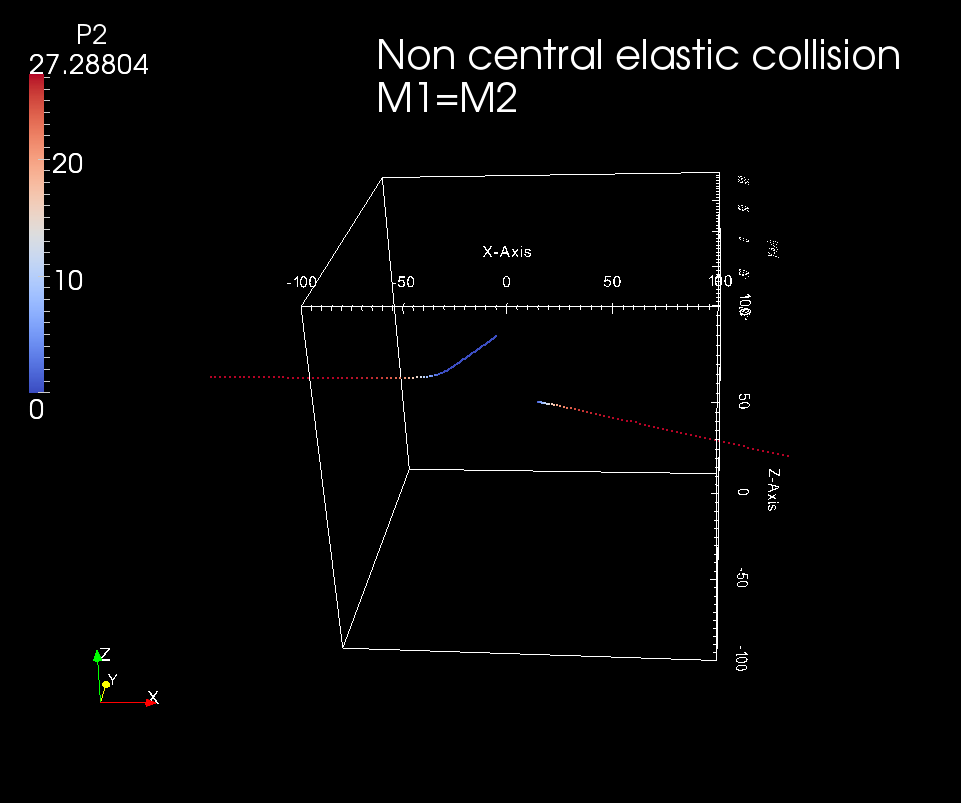
\includegraphics{graphics/central3.png}

%%%%%%%%%%%%%%%%%%%%%%
}

\begin{equation}
X_i(t+ \bigtriangleup t)=F_i(X_i(t)) \;\; (i \in 1..N)
 \label{eq:iteration}
\end{equation}

The algorithm is straight forward and it shows clearly this loop 
may be executed in parallel on multiple processors sine the calculation 
may be brocken down in indendant partitions.

\begin{algorithm}
\caption{A loop algoritm}
\label{alg:loop}
\begin{algorithmic}
\For { $i \in 1..N$ }
    \State{ $X1(i) \gets{F(i,X0)} $ }
\EndFor
\end{algorithmic}
\end{algorithm}

Paraffin provides for such an problem so called paralell loops. \autoref{lst:example1}
shows the implementation of equation \autoref{eq:iteration}. The main element of the 
caculation is the function F which computes the value of \begin{math} 
X_i(t+ \bigtriangleup t) \end{math} for all \begin{math}i \in 1..N\end{math}. 
This function is called by the function Do{\textunderscore}Partition which in turn is called by Paraffin with the smallest and the largest component to be calculated.

 
\begin{listing}
\lstinputlisting[caption={Parallel processing of a state vector},
       label={lst:example1},
       frame=single, 
       captionpos=b, 
       language=Ada]
    {"example/example1.adb"}
\end{listing}

\end{document}s